\documentclass[a4paper, 12pt]{extarticle}

% Поля
%--------------------------------------
\usepackage{geometry}
\geometry{a4paper,tmargin=2cm,bmargin=2cm,lmargin=3cm,rmargin=1cm}
%--------------------------------------


%Russian-specific packages
%--------------------------------------
\usepackage[T2A]{fontenc}
\usepackage[utf8]{inputenc} 
\usepackage[english, main=russian]{babel}
%--------------------------------------

\usepackage{textcomp}

% Красная строка
%--------------------------------------
\usepackage{indentfirst}               
%--------------------------------------             


%Graphics
%--------------------------------------
\usepackage{graphicx}
\graphicspath{ {./images/} }
\usepackage{wrapfig}
\usepackage{minted}
%--------------------------------------

% Полуторный интервал
%--------------------------------------
\linespread{1.3}                    
%--------------------------------------

%Выравнивание и переносы
%--------------------------------------
% Избавляемся от переполнений
\sloppy
% Запрещаем разрыв страницы после первой строки абзаца
\clubpenalty=10000
% Запрещаем разрыв страницы после последней строки абзаца
\widowpenalty=10000
%--------------------------------------

%Списки
\usepackage{enumitem}

%Подписи
\usepackage{caption} 

%Гиперссылки
\usepackage{hyperref}

\hypersetup {
	unicode=true
}

%Рисунки
%--------------------------------------
\DeclareCaptionLabelSeparator*{emdash}{~--- }
\captionsetup[figure]{labelsep=emdash,font=onehalfspacing,position=bottom}
%--------------------------------------

\usepackage{tempora}
\usepackage{amsmath}
\usepackage{color}
\usepackage{listings}
\lstset{
  belowcaptionskip=1\baselineskip,
  breaklines=true,
  frame=L,
  xleftmargin=\parindent,
  language=Python,
  showstringspaces=false,
  basicstyle=\footnotesize\ttfamily,
  keywordstyle=\bfseries\color{blue},
  commentstyle=\itshape\color{purple},
  identifierstyle=\color{black},
  stringstyle=\color{red},
}

%--------------------------------------
%			НАЧАЛО ДОКУМЕНТА
%--------------------------------------

\begin{document}

%--------------------------------------
%			ТИТУЛЬНЫЙ ЛИСТ
%--------------------------------------
\begin{titlepage}
\thispagestyle{empty}
\newpage


%Шапка титульного листа
%--------------------------------------
\vspace*{-30 pt}
\hspace{-65pt}
\begin{minipage}{0.3\textwidth}
\hspace*{-20pt}\centering

\includegraphics[width=60pt]{emblem}
\end{minipage}
\begin{minipage}{0.67\textwidth}\small \textbf{
\vspace*{-0.7ex}
\hspace*{-6pt}\centerline{Министерство науки и высшего образования Российской Федерации}
\vspace*{-0.7ex}
\centerline{Федеральное государственное бюджетное образовательное учреждение }
\vspace*{-0.7ex}
\centerline{высшего образования}
\vspace*{-0.7ex}
\centerline{<<Московский государственный технический университет}
\vspace*{-0.7ex}
\centerline{имени Н.Э. Баумана}
\vspace*{-0.7ex}
\centerline{(национальный исследовательский университет)>>}
\vspace*{-0.7ex}
\centerline{(МГТУ им. Н.Э. Баумана)}}
\end{minipage}
%--------------------------------------

\vspace{10pt}
\hspace{-35pt} \noindent \small ФАКУЛЬТЕТ\hspace{80pt} <<Информатика и системы управления>>

\vspace*{-16pt}
\hspace{47pt}\rule{0.83\textwidth}{0.4pt}

\vspace{0.5ex}
\hspace{-35pt} \noindent \small КАФЕДРА\hspace{50pt} <<Теоретическая информатика и компьютерные технологии>>

\vspace*{-16pt}
\hspace{30pt}\rule{0.866\textwidth}{0.4pt}
  
\vspace{6em}

\begin{center}
\Large {\bf Лабораторная работа №6} \\ 
\large {\bf по курсу <<Языки и методы программирования>>} \\ 
\large «Программа с графическим пользовательским интерфейсом» \\
\large <<Вариант 26>>
\end{center}\normalsize

\vspace{15em}


\begin{flushright}
  {Студент группы ИУ9-21Б: Пенкин А. Д.\hspace*{15pt} \\
  \vspace{2ex}
  Преподаватель: Посевин Д. П.\hspace*{15pt}}
\end{flushright}

\bigskip

\vfill
 \vspace{7em}

\begin{center}
\textsl{Москва 2023}
\end{center}
\end{titlepage}
%--------------------------------------
%		КОНЕЦ ТИТУЛЬНОГО ЛИСТА
%--------------------------------------

\renewcommand{\ttdefault}{pcr}

\setlength{\tabcolsep}{3pt}
\newpage
\setcounter{page}{2}

\section{Цель}\label{Sect::task}
\par
Приобретение навыков разработки программ с графическим пользовательским интерфейсом на основе библиотеки swing. 
\section{Условие}
\par
Продемонстрируем создание приложения с графическим пользовательским интерфейсом в IntelliJ IDEA на примере простой программы, рисующей бутылку, имеющую высоту h и диаметр d, с горлышком длины h=3 и диаметром d=3, заполненная жидкостью на k процентов.
\section{Код решения}
1. PictureForm.java
\begin{minted}{java}
import javax.swing.*;
import javax.swing.event.ChangeEvent;
import javax.swing.event.ChangeListener;


public class PictureForm {
    private JPanel mainPanel;
    private JSpinner ширинаSpinner;
    private JSpinner высотаSpinner;
    private JSpinner процентЗаполненностиSpinner;
    private JTextPane percentPanel;
    private CanvasPanel canvasPanel1;

    public PictureForm() {
        процентЗаполненностиSpinner.addChangeListener(new ChangeListener() {
            @Override
            public void stateChanged(ChangeEvent e) {
                int percent = (int)процентЗаполненностиSpinner.getValue();
                if (percent >= 100) {
                    процентЗаполненностиSpinner.setValue(100);
                    percent=100;
                }
                if (percent <= 0) {
                    процентЗаполненностиSpinner.setValue(0);
                    percent=0;
                }
                int V = (int)((double) percent / 400 * 3.1415 *
                        (int)ширинаSpinner.getValue() *
                        (int)ширинаSpinner.getValue() *
                        (int) высотаSpinner.getValue());
                percentPanel.setText(String.format("Объём: %d", V));
                canvasPanel1.setPercent(percent);
            }
        });
        высотаSpinner.addChangeListener(new ChangeListener() {
            @Override
            public void stateChanged(ChangeEvent e) {
                int hight = (int)высотаSpinner.getValue();
                if (hight <= 1){
                    высотаSpinner.setValue(1);
                    hight = 1;
                }
                if (hight >= 45){
                    высотаSpinner.setValue(45);
                    hight = 45;
                }
                canvasPanel1.setHight(hight);
                int V = (int)((double) (int)процентЗаполненностиSpinner.getValue()
                        / 400 * 3.1415 *
                        (int)ширинаSpinner.getValue() *
                        (int)ширинаSpinner.getValue() *
                        (int) высотаSpinner.getValue());
                percentPanel.setText(String.format("Объём: %d", V));
            }
        });
        ширинаSpinner.addChangeListener(new ChangeListener() {
            @Override
            public void stateChanged(ChangeEvent e) {
                int width = (int)ширинаSpinner.getValue();
                if (width <= 1){
                    ширинаSpinner.setValue(1);
                    width = 1;
                }
                if (width >= 38){
                    ширинаSpinner.setValue(38);
                    width = 38;
                }
                int V = (int)((double) (int)процентЗаполненностиSpinner.getValue()
                        / 400 * 3.1415 *
                        (int)ширинаSpinner.getValue() *
                        (int)ширинаSpinner.getValue() *
                        (int) высотаSpinner.getValue());
                percentPanel.setText(String.format("Объём: %d", V));
                canvasPanel1.setDiameter(width);
            }
        });

        ширинаSpinner.setValue(7);
        canvasPanel1.setDiameter(7);
        высотаSpinner.setValue(20);
        процентЗаполненностиSpinner.setValue(95);

    }

    public static void main(String[] args) {
        JFrame frame = new JFrame("Bottle");
        frame.setContentPane(new PictureForm().mainPanel);
        frame.setDefaultCloseOperation(JFrame.EXIT_ON_CLOSE);
        frame.pack();
        frame.setVisible(true);
    }

    private void createUIComponents() {
        canvasPanel1 = new CanvasPanel();
    }
}
\end{minted}
2. CanvasPanel.java
\begin{minted}{java}
import javax.swing.*;
import java.awt.*;

public class CanvasPanel extends JPanel {
    private int diameter = 7, hight = 20, percent = 95;

    public void setDiameter(int newd){
        diameter = newd;
        repaint();
    }
    public void setHight(int newd){
        hight = newd;
        repaint();
    }
    public void setPercent(int newd){
        percent = newd;
        repaint();
    }
    protected void paintComponent (Graphics g) {
        super.paintComponent(g);
        g.setColor(Color.green);
        g.fillRoundRect(185, 10, 30, 30, 1, 1);
        g.fillRoundRect(200 - diameter * 5, 40,
                diameter * 10, hight * 10, 10, 5);
        g.setColor(Color.pink);
        g.fillRoundRect(200 - diameter * 5,
                40 + (int)((float)hight * ((float)(100 - percent) / 10)),
                diameter * 10,
                (int)((float)hight * percent / 10), 10 ,5);
    }
}
\end{minted}

\section{Результаты работы программы}
\begin{figure}[H]
    \centering
    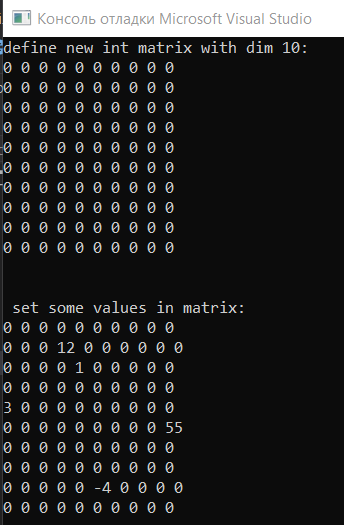
\includegraphics[width=400pt]{Test.png}
    \caption{форма в IntelliJ IDEA}
    \label{fig:my_label}
\end{figure}

\begin{figure}[H]
    \centering
    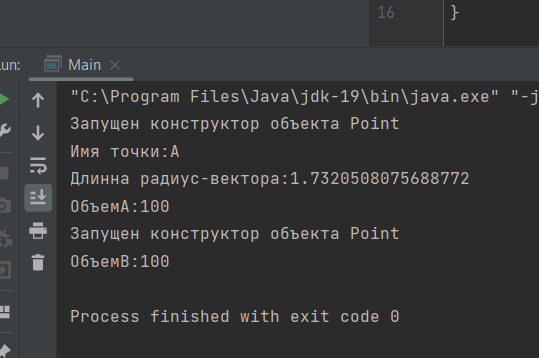
\includegraphics[width=400pt]{Test1.png}
    \caption{запуск программы, стартовая панель}
    \label{fig:my_label}
\end{figure}

\begin{figure}[H]
    \centering
    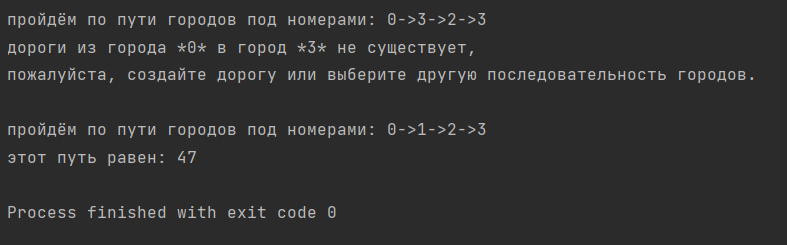
\includegraphics[width=400pt]{Test2.png}
    \caption{изменение параметров}
    \label{fig:my_label}
\end{figure}


\end{document}